\chapter{Rendering}
\label{ch:rendering}

Per la fase di rendering viene utilizzato Blender, sia tramite uno script Python basato sulle API \texttt{bpy}, sia tramite la sua interfaccia grafica (GUI).

Il file GLTF esportato dalla pipeline (Sezione \ref{sec:esportazione}) contiene esclusivamente la geometria della mesh (posizioni, normali e coordinate texture) e non include alcuna informazione sui materiali. I materiali, così come gli asset di porte e finestre e l'environment map, vengono quindi definiti direttamente in Blender. In questo modo è possibile, ad esempio, cambiare le texture senza dover rieseguire ogni volta l'intera pipeline.

\section{Generazione della scena}
\label{sec:generazione_scena_blender}

Inizialmente si era valutato di eseguire l'intero rendering all'interno dello script Python. Questo approccio si è tuttavia rivelato poco pratico: posizione e rotazione della camera, così come posizione e intensità delle luci, avrebbero dovuto essere codificate direttamente nel codice (\emph{hard-coding}), rendendo la scelta dei parametri laboriosa e poco intuitiva. Si è quindi adottato un approccio ibrido: lo script Python automatizza le operazioni ripetitive e deterministiche, mentre la composizione finale della scena (camera e luci) è affidata alla GUI di Blender.

Lo script esegue, in ordine, le seguenti operazioni:

\begin{enumerate}
	\item importazione del modello GLTF;
	\item definizione dei materiali (albedo, normal, roughness, ecc.) per il pavimento e per i muri;
	\item impostazione dell'environment map;
	\item caricamento degli asset di porte e finestre e loro posizionamento in corrispondenza delle aperture, a partire dalle informazioni contenute nel file JSON dei varchi (Sezione \ref{sec:esportazione});
	\item creazione di alcune luci iniziali;
	\item salvataggio della scena in un file \texttt{.blend}.
\end{enumerate}

Il posizionamento degli asset si basa sul file \texttt{*\_openings.json}, generato in fase di esportazione insieme al modello GLTF (Sezione \ref{sec:esportazione}). Per ciascun varco, il file contiene tutte le informazioni necessarie: il tipo (\texttt{DOOR} o \texttt{WINDOW}), il centro, la larghezza, l'altezza, lo spessore e la rotazione attorno all'asse verticale (\texttt{rotation\_z}). Lo script utilizza il tipo per scegliere quale asset caricare, il centro e la rotazione per posizionarlo e orientarlo, e le dimensioni per scalarlo in modo che si adatti esattamente all'apertura.


\section{Setup della scena e rendering}
\label{sec:setup_scena}

Il file \texttt{.blend} generato viene aperto in Blender tramite GUI, e comprende mesh, asset, materiali ed environment map. In questa modalità, l'impostazione della camera risulta molto più comoda: è possibile navigare liberamente nella scena, posizionare opportunamente le luci e modificarne le proprietà.

Il rendering fotorealistico viene eseguito con il motore Cycles, un path tracer fisicamente basato che simula il trasporto della luce nella scena, compresa l'illuminazione globale. Il rendering è stato effettuato a risoluzione $1280 \times 720$, con 128 campioni per pixel e denoiser attivo, il quale riduce il rumore residuo tipico dei metodi Monte Carlo e consente di utilizzare un numero contenuto di campioni.

Il rendering è stato eseguito esclusivamente su CPU (AMD Ryzen 5 2600X), poiché la GPU a disposizione (AMD Radeon RX 590) non risulta utilizzabile per il path tracing con Cycles. Anche il denoiser utilizzato, OpenImageDenoise, viene eseguito su CPU ed è impostato in qualità \emph{High}. Il tempo di rendering varia in funzione della complessità della scena: una scena vuota con poche luci richiede circa 3 minuti, mentre l'aggiunta di asset e sorgenti luminose lo porta a circa 6-7 minuti.

\section{Risultati}
\label{sec:risultati_rendering}

La Figura~\ref{fig:rendering_base} mostra il rendering della scena base: la geometria generata dalla pipeline, con materiali, asset di porte e finestre ed environment map.
\begin{figure}[htbp]
	\centering
	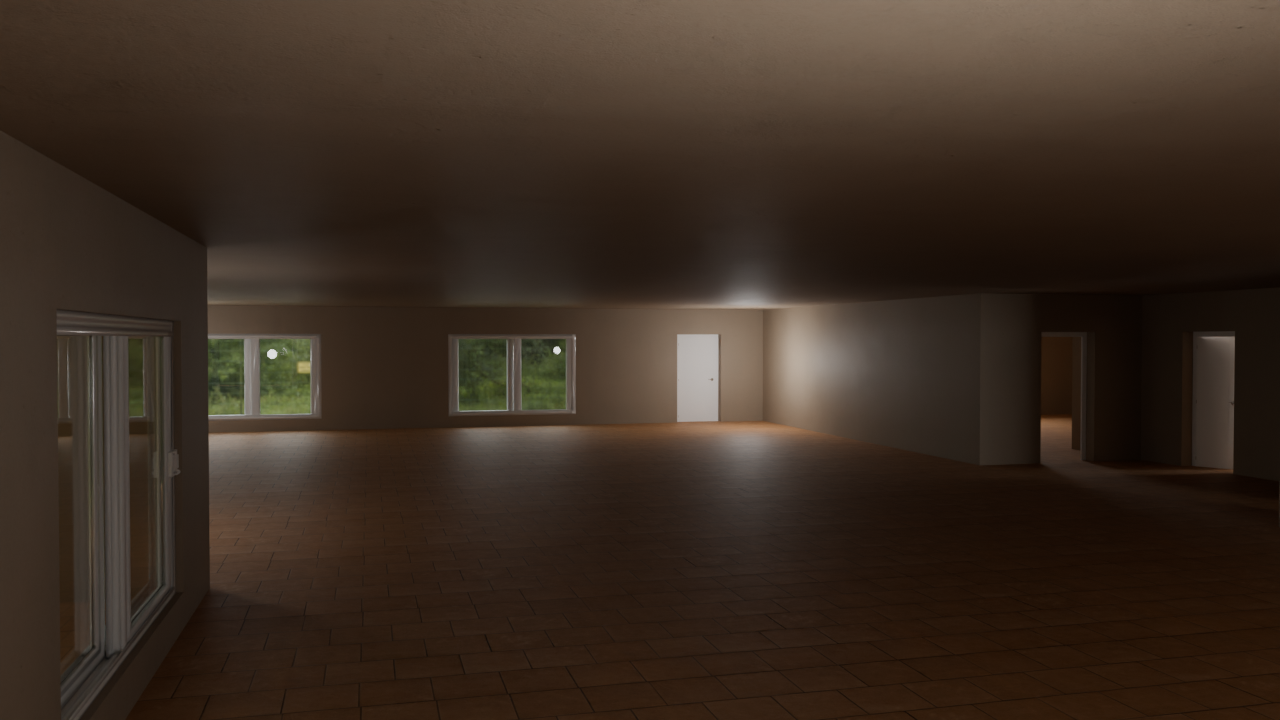
\includegraphics[width=1\textwidth]{figures/4_rendering/draftperson_HousePlan-rendering-1280x720-128-1.png}
	\caption{Rendering della scena base con Cycles ($1280 \times 720$, 128 campioni per pixel, denoiser attivo).}
	\label{fig:rendering_base}
\end{figure}

Come si osserva, la scena risulta piuttosto spoglia. Grazie alla modalità GUI è possibile aggiungere facilmente ulteriori asset per arredarla, come un divano, una TV, una lampada o un letto. Le figure seguenti mostrano alcuni esempi di scene arredate.
\begin{figure}[htbp]
	\centering
	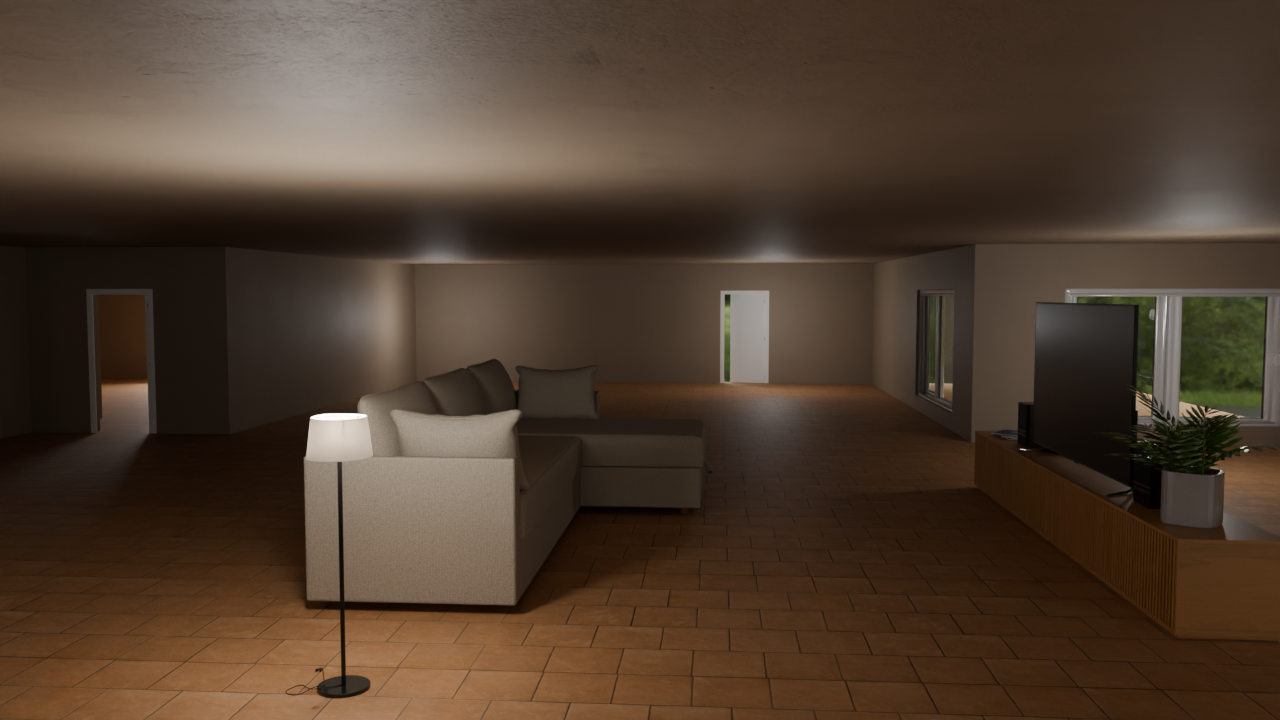
\includegraphics[width=1\textwidth]{figures/4_rendering/draftperson_HousePlan-rendering-1280x720-128-2.png}
	\caption{Scena arredata: soggiorno con divano, TV, lampada}
	\label{fig:rendering_arredato_1}
\end{figure}
\begin{figure}[htbp]
	\centering
	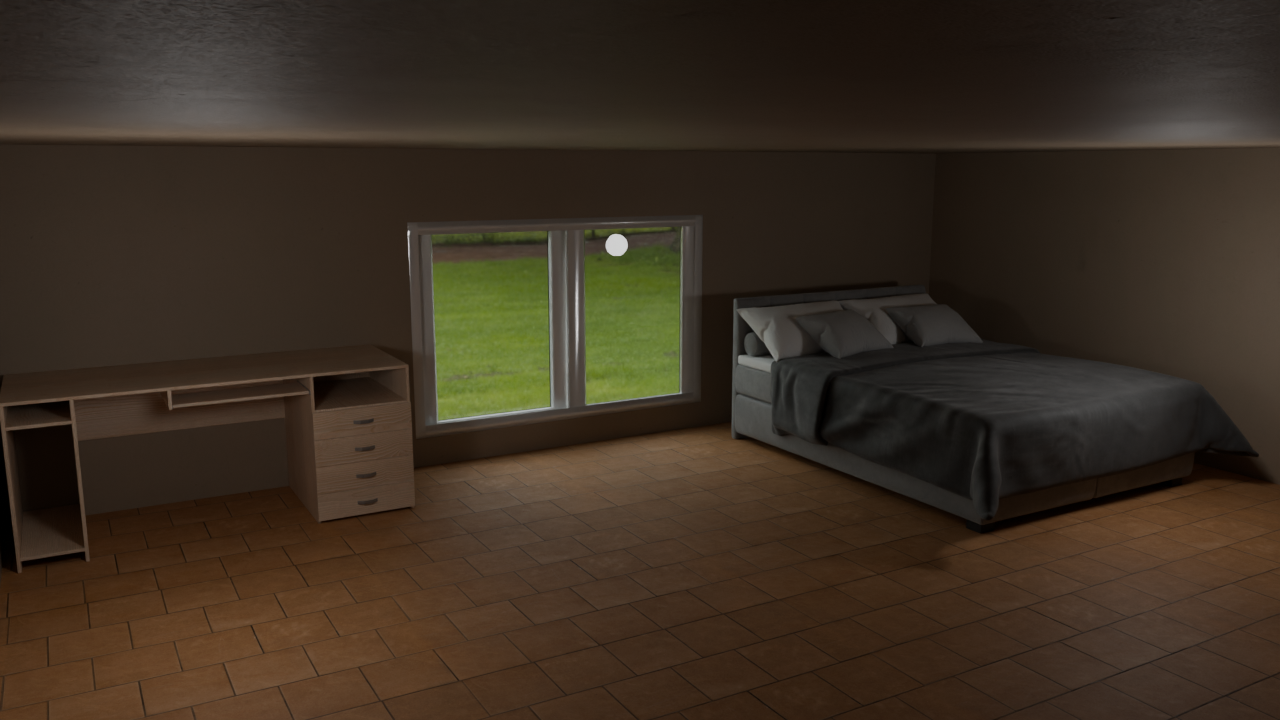
\includegraphics[width=1\textwidth]{figures/4_rendering/draftperson_HousePlan-rendering-1280x720-128-3.png}
	\caption{Scena arredata: camera da letto con una scrivania e un letto}
	\label{fig:rendering_arredato_2}
\end{figure}
\begin{figure}[htbp]
	\centering
	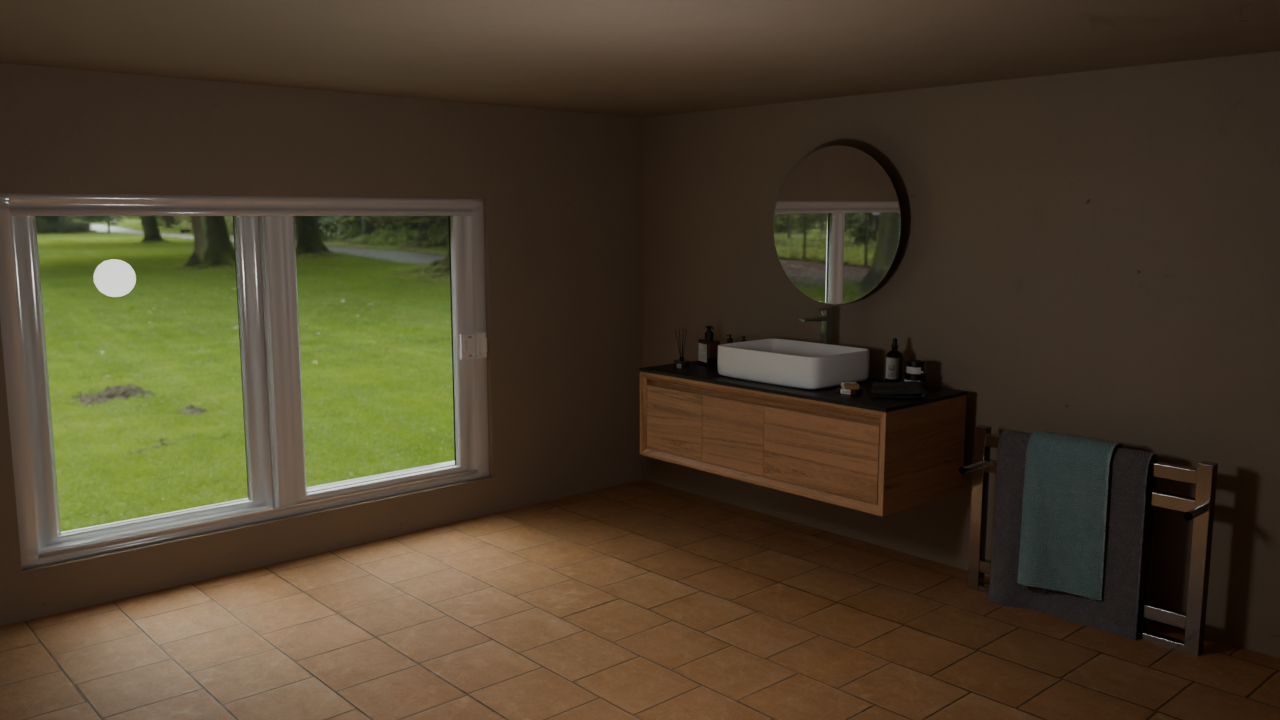
\includegraphics[width=1\textwidth]{figures/4_rendering/draftperson_HousePlan-rendering-1280x720-128-4.png}
	\caption{Scena arredata: un bagno con un lavandino, uno specchio, un asciugamano}
	\label{fig:rendering_arredato_3}
\end{figure}

\FloatBarrier

\begin{table}[htbp]
	\centering
	\caption{Statistiche dell'esecuzione della pipeline.}
	\label{tab:statistiche_caso_1}
	\begin{tabular}{lr}
		\hline
		Segmenti duplicati rimossi (finestre) & 64 \\
		Segmenti totali (muro / porta / finestra) & 88 / 4 / 113 \\
		Vertici 2D totali (tutti i segmenti) & 410 \\
		Vertici sui muri prima dello snapping & 176 \\
		Vertici sui muri dopo lo snapping & 88 \\
		Vertici collassati & 88 \\
		Vertici univoci nel grafo finale (2D) & 88 \\
		Punti campionati per il clustering & 3503 \\
		Cluster individuati (finestre) & 8 \\
		Facce di muro & 10 \\
		Facce di porta & 4 \\
		Facce di finestra & 8 \\
		Vertici mesh (3D) & 804 \\
		Indici mesh & 1140 \\
		Tempo di esecuzione della pipeline & 5,7 s \\
		\hline
	\end{tabular}
\end{table}